% Don't touch this %%%%%%%%%%%%%%%%%%%%%%%%%%%%%%%%%%%%%%%%%%%
\documentclass[11pt]{article}
\usepackage{fullpage}
\usepackage[left=1in,top=1in,right=1in,bottom=1in,headheight=3ex,headsep=3ex]{geometry}
\usepackage{graphicx}
\usepackage{float}
\renewcommand{\theenumi}{\Alph{enumi})}

\newcommand{\blankline}{\quad\pagebreak[2]}
%%%%%%%%%%%%%%%%%%%%%%%%%%%%%%%%%%%%%%%%%%%%%%%%%%%%%%%%%%%%%%

% Modify Course title, instructor name, semester here %%%%%%%%

\title{\textbf{GGR424: Transportation Geography \& Planning}}
\author{Jeff Allen}
\date{Winter, 2022}

%%%%%%%%%%%%%%%%%%%%%%%%%%%%%%%%%%%%%%%%%%%%%%%%%%%%%%%%%%%%%%

% Don't touch this %%%%%%%%%%%%%%%%%%%%%%%%%%%%%%%%%%%%%%%%%%%
\usepackage[sc]{mathpazo}
\linespread{1.05} % Palatino needs more leading (space between lines)
\usepackage[T1]{fontenc}
\usepackage[mmddyyyy]{datetime}% http://ctan.org/pkg/datetime
\usepackage{advdate}% http://ctan.org/pkg/advdate
\newdateformat{syldate}{\twodigit{\THEMONTH}/\twodigit{\THEDAY}}
\newsavebox{\MONDAY}\savebox{\MONDAY}{Mon}% Mon
\newcommand{\week}[1]{%
	%  \cleardate{mydate}% Clear date
	% \newdate{mydate}{\the\day}{\the\month}{\the\year}% Store date
	\paragraph*{\kern-2ex\quad #1, \syldate{\today} - \AdvanceDate[4]\syldate{\today}:}% Set heading  \quad #1
	%  \setbox1=\hbox{\shortdayofweekname{\getdateday{mydate}}{\getdatemonth{mydate}}{\getdateyear{mydate}}}%
	\ifdim\wd1=\wd\MONDAY
	\AdvanceDate[7]
	\else
	\AdvanceDate[7]
	\fi%
}
\usepackage{setspace}
\usepackage{multicol}
%\usepackage{indentfirst}
\usepackage{fancyhdr,lastpage}
\usepackage{url}
\pagestyle{fancy}
\usepackage{hyperref}
\usepackage{lastpage}
\usepackage{amsmath}
\usepackage{layout}

\lhead{}
\chead{}
%%%%%%%%%%%%%%%%%%%%%%%%%%%%%%%%%%%%%%%%%%%%%%%%%%%%%%%%%%%%%%

% Modify header here %%%%%%%%%%%%%%%%%%%%%%%%%%%%%%%%%%%%%%%%%
\rhead{\footnotesize Transportation Data Analysis | GGR424}
\lhead{\footnotesize Jeff Allen}
%%%%%%%%%%%%%%%%%%%%%%%%%%%%%%%%%%%%%%%%%%%%%%%%%%%%%%%%%%%%%%
% Don't touch this %%%%%%%%%%%%%%%%%%%%%%%%%%%%%%%%%%%%%%%%%%%
\lfoot{}
\cfoot{\small \thepage/\pageref*{LastPage}}
\rfoot{}

\usepackage{array, xcolor}
\usepackage{color,hyperref}
\definecolor{clemsonorange}{HTML}{f00000}
\hypersetup{colorlinks,breaklinks,linkcolor=clemsonorange,urlcolor=clemsonorange,anchorcolor=clemsonorange,citecolor=black}

\setlength{\parindent}{0em}
\setlength{\parskip}{0.8em}

\usepackage{colortbl}
\usepackage{tabularx,ragged2e}
\usepackage{sectsty}


\usepackage{helvet}

\begin{document}
	\allsectionsfont{\sffamily}
	
	\section*{Transportation Data Analysis Assignment} 
		
	\textit{Due February 28 at 11:59pm}
	
	Please submit your assignment as \textbf{one} pdf or Word doc on Quercus before the due date. Do not upload separate maps or images. Put your name and student number in the header of your assignment.
	
	All the technical questions can be completed using Excel and/or standard GIS software (QGIS or ArcGIS). But you are free to use any other software/tools that you want for any part of this assignment (e.g. R, Python, etc.).
	
	\texttt{data.zip} contains all the data required to complete this assignment.
	
	All maps should be 6.5 inches wide (and thus fit nicely on an 8.5x11 page with 1 inch margins). Please present all maps in a projection that preserves local directions and shapes (e.g. Web Mercator, UTM Zone 17N, etc.). Rotate all maps of Toronto so that Steele Ave is parallel to the top border of the map (about 17 degrees).
	
		
	\subsection*{Part 1: Thinking About Accessibility} 
	
	\vspace{-2mm}
	\textbf{\textit{3 marks}}
	
	Consider a city with 10 neighbourhoods, each with 1,000 jobs, that are connected with a single transit line. Assume that the travel time between each adjacent stop is \textbf{10 minutes} and that the headway is \textbf{2 minutes}. 
	
	\begin{figure}[h]
		\centering
		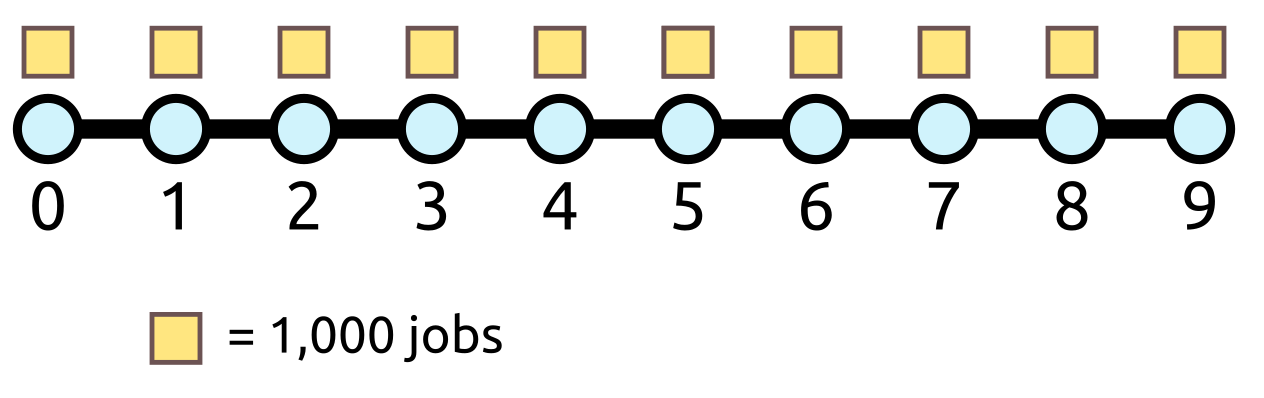
\includegraphics[width=0.5\linewidth]{images/city_plain.png}
	\end{figure}

	The city has grown recently, use your student number to distribute where employment growth is located in the city. Do this by allocating 1,000 additional jobs to each neighbourhood for each digit in your student number.
	
	Answer the following questions based on your student number:
	
	\begin{enumerate}
		
		
		\item If you live in neighbourhood \textbf{0}, how many jobs can you reach in less than or equal to a \textbf{45} minute transit trip? (1) 
		
		\item Using this travel time threshold (\textbf{45} minutes), which neighbourhood(s) has the greatest level of accessibility to jobs? (1) 
		
		\item The city is planning to build a high speed express route to directly connect the stops in neighbourhood \textbf{0} and neighbourhood \textbf{9} in only \textbf{30} minutes (it will also have a headway of \textbf{2} minutes). If you still live in neighbourhood \textbf{0}, how many jobs will you then be able to access in a \textbf{45} minute trip? (1) 
		
	\end{enumerate}

	(For example, if your student number is 2013455888, then the distribution of jobs in the city would be as follows)
	
	\begin{figure}[h]
		\centering
		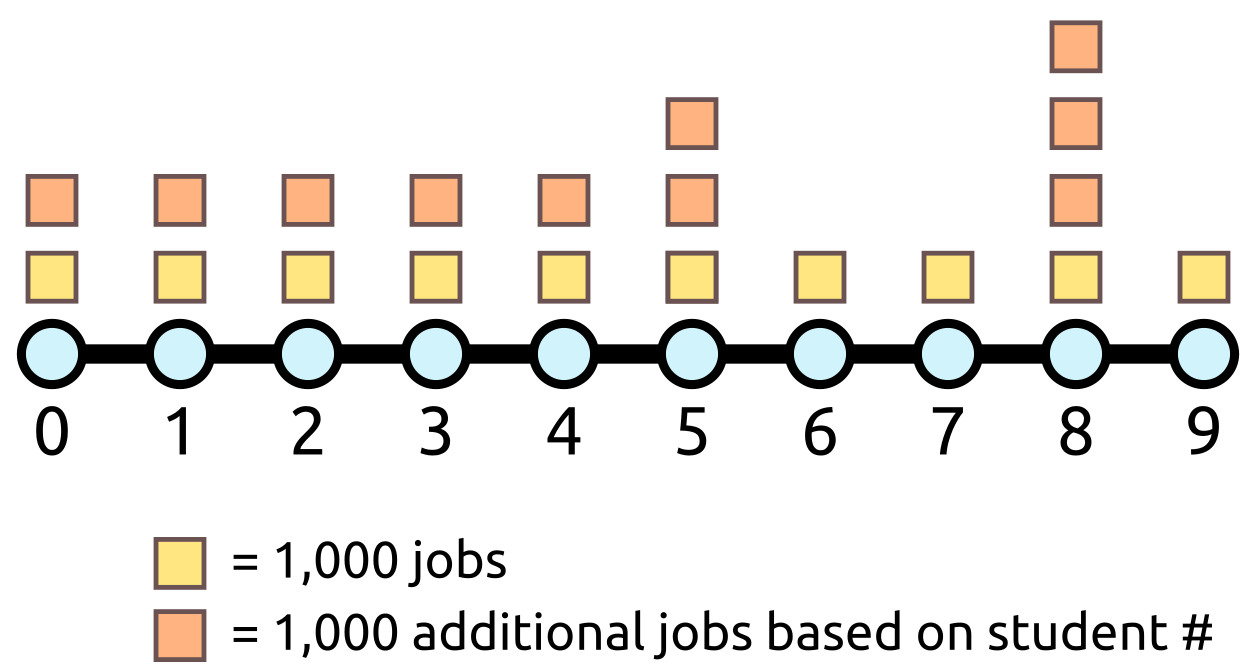
\includegraphics[width=0.5\linewidth]{images/city_jobs.png}
	\end{figure}
	
	
	\subsection*{Part 2: Mapping Cycling}
	
	\vspace{-2mm}
	\textbf{\textit{7 marks}}
	
	You've been tasked with analyzing where cycling infrastructure is related to cycling mode share in Toronto. 
	
	Cycling mode share for journey to work trips. In \texttt{data.zip}, there are geojson files for bicycle infrastructure and bikeshare stations.
	
	
	\begin{enumerate}	
		\item Create a map with bicycle infrastructure and bike-share stations overlaid on top of a choropleth map of cycling mode share by census tract. (3 marks)
		
		\item Describe in 2-4 sentences the patterns between the layers. 
		
		Where in the city (1.5 marks)
		
		\item Limited data () (2.5 marks), A network dataset of cycling in Toronto
		
	\end{enumerate}
	
	
	
	
	
	\subsection*{Part 3: Pedestrian Accessibility To Libraries} 
	
	\textbf{\textit{6 marks}}
	
	Compute service areas for walking for public libraries
	
	Create two maps, one overlaid with population dot density, one with low-income population density 
	
	(4 marks)
	
	Breifly describe patterns, etc.
	
	(2 marks)

	
	
	
	\subsection*{Part 4: Transit Accessibility To Employment}
	
	\textbf{\textit{6 marks)}}
	
	
	Given OD matrix of DAs (describe creation)
	
	Measure access to jobs in 45 minutes
	
	Create a choropleth map of transit accessibility to jobs overlaid with the line and point files of subway lines and stops. (3.5 marks)
	
	Briefly describe the pattern on the map (1 marks), as expected?
	
	Discuss limitations in this measure (1.5 marks)
	
	
	
	
	\subsection*{Part 5: Mapping Travel Choices}
	
	\textbf{\textit{7 marks}}
	
	1.5x3 + 2.5 = 7 marks
	
	1 map - Transit mode share
	
	1 map - Activity participation
	
	1 map - Commute times
	
	Qualitative response to the above  (2.5 marks)

	
	
	
	
	
	
\end{document}